\title{CS531 Programming Assignment 1: Vacuum-Cleaning Agents}
\author{
        Michael Lam, Shell Hu \\
        EECS, Oregon State University\\
        %\email{}
        %\and
}

\documentclass[12pt]{article}
\usepackage[english]{babel}
\usepackage{graphicx}
\usepackage{subfig}
\usepackage{amsmath}
\usepackage{hyperref}
\hypersetup{
    colorlinks,%
    citecolor=green,%
    filecolor=magenta,%
    linkcolor=red,%
    urlcolor=cyan
}

%\underset{x}{\operatorname{argmax}}
%\underset{x}{\operatorname{argmin}}
\DeclareMathOperator*{\argmin}{arg\,min}
\DeclareMathOperator*{\argmax}{arg\,max}

\begin{document}
\maketitle

\begin{abstract}
In this assignment you design and implement 3 different vacuum-cleaning agents.
\end{abstract}

% -------------------------------------------------
\section{Introduction}

Consider an environment where the world is a rectangular room consisting of $ n \times m $ cells, with each cell having a probability of dirt. There are three vacuum cleaner agents in consideration: 1) memoryless deterministic reflex agent, 2) randomized reflex agent, and 3) deterministic model-based reflex agent with 3 bits of memory. The agent has three percepts (wall, dirt, home) and five actions (forward, right, left, suck, turn off). The performance measure is the total number of clean cells as a function of how many action steps were taken. We also would like the agent to return to its home cell and shut off after it cleans the entire room.

Having described the environment, agent and performance measure, the general goal of a successful vacuum cleaner agent is to clean the entire room in a minimal number of steps. While that is the ideal case, two of our agents are not able to satisfy this goal. Thus we have different goals for our agents due to their designs by definition. The first agent in consideration, the memoryless deterministic reflex agent, is limited by pure reflex actions with no memory. We discovered that we cannot clean every cell with this agent, so our goal for this agent is to clean as many cells as possible and to return home at the end. For the randomized reflex agent, its performance is improved and simultaneously hindered by its probabilistic actions. We discovered that while it can clean the entire room over time, it is difficult to maneuver the agent back to the home cell due to randomness. The goal for this agent then is to clean every cell without needing to return home. Finally, the deterministic model-based reflex agent has memory, which gives it advantage to remember which actions it has taken. Given this advantage, the goal of this agent is to clean the entire room and navigate home successfully. We determined that this was possible in less than 8 states, the maximum cap for the agent's memory.

\section{Simple Memoryless Deterministic Reflex Agent}

\section{Randomized Reflex Agent}

\section{Deterministic Model-Based Agent}

Since the deterministic model-based reflex agent has some memory to store state information, we exploit this property to design a better agent that can 1) suck up dirt at every square (which fails for the memoryless reflex agent) and 2) get home properly (which fails for the randomized reflex agent).

\subsection{Design Considerations}

The requirements of the deterministic model-based reflex agent other than its definition is that it can represent state with only 3 bits of memory, which implies up to 8 states\footnote{Without loss of generality, we can use one state variable STATE that takes on integers $[0, 7]$ instead of three explicit state bits STATE1, STATE2 and STATE3 because $0 = 000, 1 = 001, 2 = 010, ..., 7 = 111$.}. We want the agent to suck every dirt as our first goal. Since the agent has memory, we are able to perform two ``consecutive'' actions by taking advantage of state information. This will allow the agent to steer into the middle of the world in contrast to the simple memoryless reflex agent, which could only suck dirt near the boundaries of the world.

In addition, our second goal is to incorporate a method for the agent to return home after it has cleaned every cell. We can use state information to represent the state ``done cleaning.'' In fact, we will show that in our design, only one state in addition to the percept is sufficient to steer home.

Therefore, we designed an algorithm to clean every cell and return home systematically since our agent is deterministic and has memory. We designed the algorithm so that our agent performs the sweeping pattern across the room as in figure \ref{fig:motion}.

\begin{figure}[!t]
	\centering
	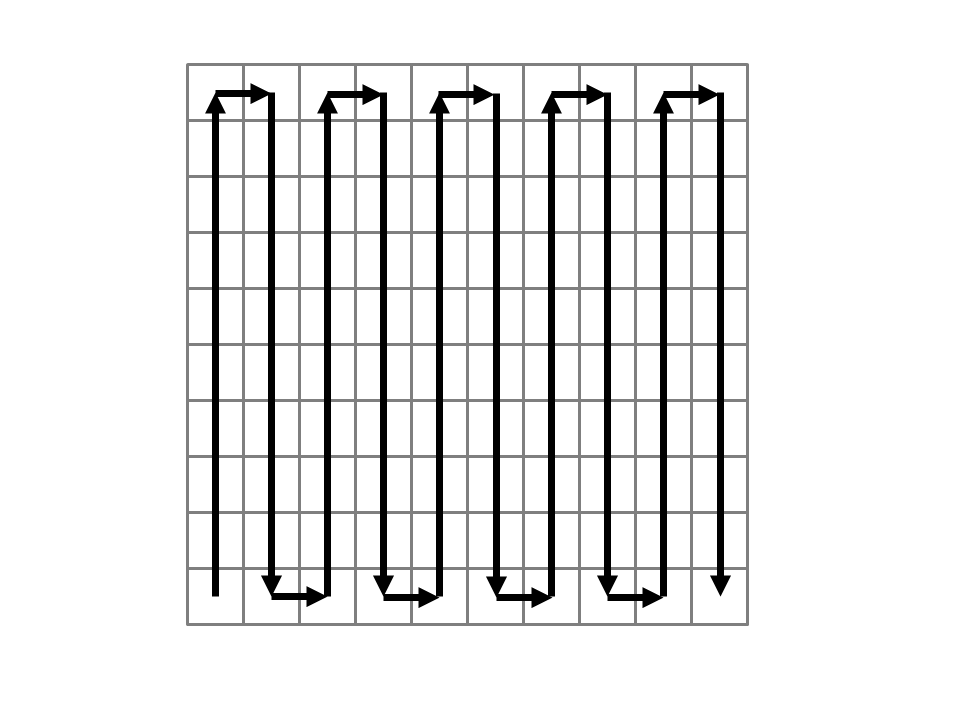
\includegraphics[scale=.30]{img/3-motion.png}
	\caption{The deterministic model-based reflex agent starts at the bottom-left corner and sweeps north, east, south, east, etc. as shown in the figure.}
	\label{fig:motion}
\end{figure}

\begin{figure}[!t]
	\centering
	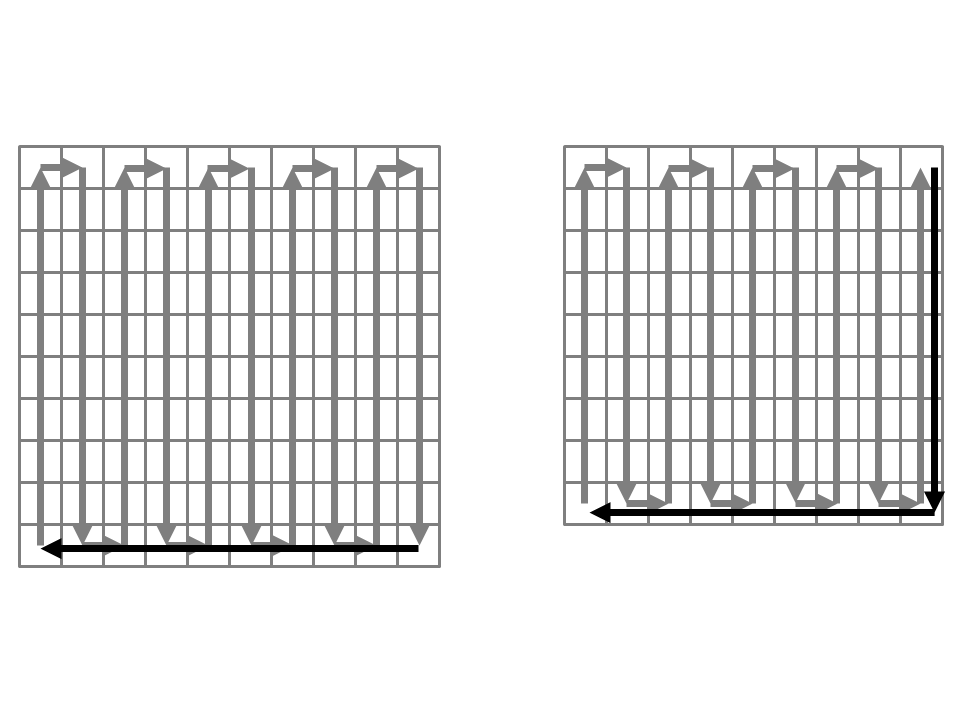
\includegraphics[scale=.30]{img/3-motionend.png}
	\caption{Once the agent is done cleaning, it moves to state 6, which is just a series of reflex actions similar to the memoryless agent. In the case when the agent is done cleaning at the top-right corner (left figure), it moves south and then west back to the home cell along the world boundaries. In the case when the agent is done cleaning at the bottom-right corner (right figure), it moves west back to the home cell along the world boundary.}
\end{figure}

\subsection{Algorithm and Rules}

Our agent performs the following algorithm: 

\begin{enumerate}
	\item Begin at the home cell.
	\item Go north and suck until it hits the south boundary. 
	\item Go one cell east.
	\item Go south and suck until it hits the south boundary.
	\item Go one cell east.
	\item Repeat steps 2-5 until there is a wall that prevents going one cell east.
	\item Traverse the world boundary until it comes home.
\end{enumerate}

We can construct the algorithm by using 7 states. We illustrate the state machine in figure \ref{fig:states}.

\begin{figure}[!t]
	\centering
	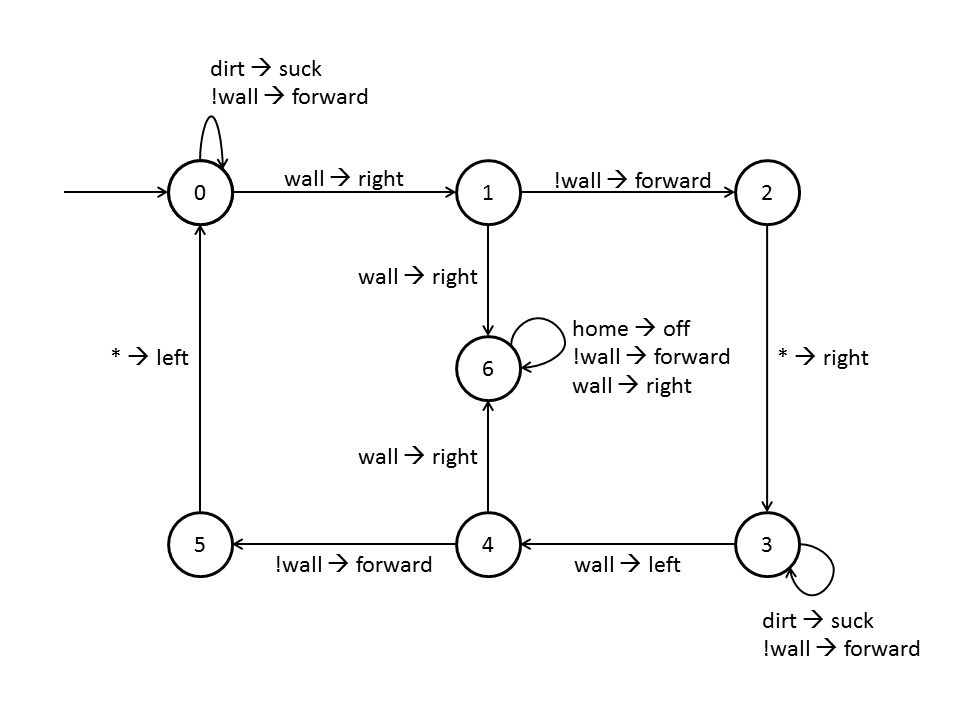
\includegraphics[scale=.30]{img/3-statediag.png}
	\caption{State machine of the model-based reflex agent.}
	\label{fig:states}
\end{figure}

In plain language and referencing figure \ref{fig:states}, state 0 represents a series of reflex actions for sucking and moving north. When the agent hits the top boundary of the world, states 1-2 assist the agent in moving east one square to prepare sucking and moving south. State 3 (symmetric to state 0) represents a series of reflex actions for sucking and moving south. When the agent hits the bottom boundary of the world, states 4-5 (symmetric to states 1-2) assist the agent in moving east one square to prepare sucking and moving north. The cycle repeats until the agent can no longer move east, as detected in states 1 and 4. If that is the case, then the agent moves to state 6, which is a series of reflex actions to navigate the agent around the edges of the map until it reaches home.

An alternative representation is the following formal list of if-then rules, which is equivalent to the state diagram. It is also coded into the agent as the program:

\begin{verbatim}
if STATE=0 and DIRT then SUCK
if STATE=0 and NOT WALL then FORWARD
if STATE=0 and WALL then STATE := 1, RIGHT
if STATE=1 and WALL then STATE := 6, RIGHT
if STATE=1 and NOT WALL then STATE := 2, FORWARD
if STATE=2 then STATE := 3, RIGHT
if STATE=3 and DIRT then SUCK
if STATE=3 and NOT WALL then FORWARD
if STATE=3 and WALL then STATE := 4, LEFT
if STATE=4 and WALL then STATE := 6, RIGHT
if STATE=4 and NOT WALL then STATE := 5, FORWARD
if STATE=5 then STATE := 0, LEFT
if STATE=6 and HOME then OFF
if STATE=6 and NOT WALL then FORWARD
if STATE=6 and WALL then RIGHT
\end{verbatim}

Therefore, we have also verified that the state diagram is equivalent to the algorithm. The algorithm is correct by construction of the state machine.

\section{Experiments}\label{sec:exp}

We solved all the $77$ problems. The first figure \ref{fig:nback} shows the number of backtrackings for each problem. The ``naked triple (double)'' strategy exhibits impressive performance in constraint propagations. Without such kinds of rules, there are $1/4$ problems need to use backtracking, no matter pick the most constrained slot or pick slot randomly. Meanwhile, only $2$ or $3$ problems require backtracking for the ``naked triple'' case. 

\begin{figure}[ht]
\centering
\begin{tabular}{cc}
\subfloat[Rule 1]{\includegraphics[scale=0.32]{../results/bt-r1-bt.pdf}} 
   & \subfloat[Rule 1,2]{\includegraphics[scale=0.32]{../results/bt-r1-r2-bt.pdf}}\\
\subfloat[Rule 1 + Naked double and triple]{\includegraphics[scale=0.32]{../results/bt-r1-n23-bt.pdf}} 
   & \subfloat[Rule 1,2 + Naked double and triple]{\includegraphics[scale=0.32]{../results/bt-r1-r2-n23-bt.pdf}}\\
%\subfloat[E]{\includegraphics[width=2cm]{logo}} 
%   & \subfloat[F]{\includegraphics[width=3cm]{logo}}\\
\end{tabular}
\caption{Number of backtracing with respect to each problem.}
\label{fig:nback}
\end{figure}

Next we show the problem completion in each difficulty level in table \ref{tab:dif}. From this table, we can see that the annotation for each problem are corrected approximately, except $3$ evil problems which were solved by only simple rules. For comparing the effectiveness of most constrained slot heuristic and random slot heuristic, we make the same experiment with random slot heuristic, which placed in last 4 rows in table \ref{tab:dif}. It seems these two heuristics are getting same results. We will further do experiments for this comparison on number of rules. For justifying the difficulty of problems, the average number of filled-in numbers are concerned, as shown in table \ref{tab:fill}.
\begin{table}[!h]
    \centering
    \scalebox{0.8}{
	    \begin{tabular}{|l|c|c|c|c|c|c|c|}
		\hline
		Complexity   & r1 & r1,2 & r1,2+n2 & r1,2+n3 & r1,2+n2,3 & r1,2+bt & r1,2+n2,3+bt \\ \hline
		Easy (23):   & 21 & 21 & 23 & 23 & 23 & 23 & 23 \\ \hline
		Medimum (21) & 3 & 3 & 10 & 14 & 19 & 21 & 21 \\ \hline
		Hard (18)    & 0 & 0 & 7 & 4 & 15 & 18 & 18 \\ \hline
		Evil (15)    & 3 & 3 & 4 & 3 & 8 & 15 & 15 \\ \hline
        \hline
		Easy rand:   & 21 & 21 & 23 & 23 & 23 & 23 & 23 \\ \hline
		Medimum rand & 3 & 3 & 10 & 14 & 19 & 21 & 21 \\ \hline
		Hard rand    & 0 & 0 & 7 & 4 & 15 & 18 & 18 \\ \hline
		Evil rand    & 3 & 3 & 4 & 3 & 8 & 15 & 15 \\ \hline
	    \end{tabular}
    }
    \caption{Number of complete problems in different combinations of rules. The default heuristic is the most constrained slot. However, it seems picking most constrained slot or picking random slot is the same in this case. Here, r1: rule 1, r1,2: rule1 + rule2, n2: naked double, n3: naked triple, n2,3: n2 + n3.}\label{tab:dif}
\end{table}

\begin{table}[!h]
    \centering
    \scalebox{0.9}{
	    \begin{tabular}{|l|c|c|c|c|}
		\hline
		             & easy & medimum & hard & evil \\ \hline
		average number & 34.70 & 29.05 & 26.28 & 26.13 \\ \hline
	    \end{tabular}
    }
    \caption{Average filled-in numbers for each problem level.}\label{tab:fill}
\end{table}

The number of rules being used is an important factor, we also use it to estimate the difficulty of a problem and show the average number of different kinds of rules used for each set of problems. The results is shown in table \ref{tab:rule}. The trendency is clear that more hard problems requires more number of rules. Note that for this experiment we use the combination of all rules and backtracking for making sure every problem can be solved.

\begin{table}[!h]
    \centering
    \scalebox{0.8}{
	    \begin{tabular}{|l|c|c|c|c|c|c|c|}
		\hline
		             & r1 & r2 & n2 & n3 & bt \\ \hline
		Easy (23):   & 42.26 & 0.04 & 22.00 & 12.70 & 0 \\ \hline
		Medimum (21) & 46.95 & 0.14 & 31.14 & 16.81 & 0 \\ \hline
		Hard (18)    & 49.06 & 0.33 & 32.11 & 15.94 & 0.06 \\ \hline
		Evil (15)    & 59.40 & 0 & 38.20 & 22.33 & 0.60 \\ \hline
	    \end{tabular}
    }
    \caption{Average number of rules used by problems in different levels. Here, r1: rule 1, r2: rule2, n2: naked double, n3: naked triple, bt: number of backtrackings.}\label{tab:rule}
\end{table}

We further compare with two heuristics in the number of rules being taken. Figure \ref{fig:heu} shows all pair of comparisons. By applying these two heuristics, a problem uses more or less the same number of rules. This is consistent with our experiment in number of complete problems. 

\begin{figure}[ht]
\centering
\begin{tabular}{cc}
\subfloat[Rule 1]{\includegraphics[scale=0.32]{../results/bt-r1-r2-n23-rule1.pdf}} 
   & \subfloat[Rule 2]{\includegraphics[scale=0.32]{../results/bt-r1-r2-n23-rule2.pdf}}\\
\subfloat[Naked double]{\includegraphics[scale=0.32]{../results/bt-r1-r2-n23-naked2.pdf}} 
   & \subfloat[Naked triple]{\includegraphics[scale=0.32]{../results/bt-r1-r2-n23-naked3.pdf}}\\
%\subfloat[E]{\includegraphics[width=2cm]{logo}} 
%   & \subfloat[F]{\includegraphics[width=3cm]{logo}}\\
\end{tabular}
\caption{Comparisons between most constrained slot heuristic and random slot heuristic in number of rules taken.}
\label{fig:heu}
\end{figure}
%
%\begin{table}[!h]
%    \centering
%    \scalebox{0.9}{
%	    \begin{tabular}{|l|c|c|c|c|c|c|c|}
%		\hline
%		Disks: & 4 & 5 & 6 & 7 & 8 & 9 & 10\\ \hline
%		A*/admissible & 8.8 & 11.6 & 13.95 & 16.5 & 18.6 & n/a & n/a\\ \hline
%		%A*/admissible H7 & 8.95 & 11.6 & 13.95 & 16.75 & 19.2 & 22.4 & 24.77\\ \hline
%		RBFS/admissible & 8.8 & 11.6 & 13.95 & 16.35 & 17.11 & n/a & n/a\\ \hline
%		A*/nonadmissible 1 & 8.85 & 11.85 & 14.6 & 17.5 & 20.2 & 24.1 & 27.6\\ \hline
%		RBFS/nonadmissible 1 & 8.85 & 11.85 & 15.25 & 19 & 22.21 & 26.81 & 32.25 \\ \hline
%		A*/nonadmissible 2 & 9.25 & 12.95 & 16.5 & 20.05 & 23.8 & 27.4 & 34.05\\ \hline
%		RBFS/nonadmissible 2 & 11.25 & 17.85 & 24.35 & 32.75 & 40.35 & 50.7 & 64.55\\ \hline
%	    \end{tabular}
%    }
%    \caption{Average solution length per algorithm, heuristic and disk size. n/a means unable to compute within 10 minutes for all problems. Note that some experiments failed for completing before NMAX nodes; these were not included in the average.}\label{tab:solen}
%\end{table}


\section{Discussion}
So far, we implemented three reflex agents and have shown that simple tasks can be done by carefully designed rules. However, it is not a good idea for creating an intelligent machine which has to handle many complex tasks. A better solution may let it learn how to do a certain type of tasks by itself. Actually, we can learn model parameters or mapping rules for our agents. We will try to use Q-learning for this improvement.

\bibliographystyle{plain}
\bibliography{ref}

\end{document}
This is never printed
